%%%%%%%%%%%%%%%%%%%%%%%%%%%%%%%%%%%%%%%%%%%%%%%%%%%%%%
% A Beamer template for Ritsumeikan University       %
% Author: Ming-Hao Xu (Xu Minghao)                   %
% Date:   April 2022.                                %
% LPPL Licensed.                                     %
%%%%%%%%%%%%%%%%%%%%%%%%%%%%%%%%%%%%%%%%%%%%%%%%%%%%%%

\documentclass[10pt]{beamer}
\usepackage{hyperref}

\usepackage[UTF8]{ctex}
\usepackage[T1]{fontenc}
\usepackage[backend=bibtex]{biblatex}
\addbibresource{ref.bib}

% other packages
\usepackage{latexsym,amsmath,xcolor,multicol,booktabs,calligra}
\usepackage{graphicx,pstricks,listings,stackengine,multirow}
\usefonttheme[onlymath]{serif}

\usepackage{tikz}
\usetikzlibrary{
  arrows.meta,
  calc,
  fit,
  positioning,
  quotes,
  fadings
}
\tikzset{>=latex}

\usepackage{algorithm}
\usepackage{caption}
\usepackage{algorithmicx}
\usepackage{algpseudocode}
\usepackage{bbm}
\floatname{algorithm}{Algorithm} %算法
\renewcommand{\algorithmicrequire}{\textbf{Input:}} %输入
\renewcommand{\algorithmicensure}{\textbf{Output:}} %输出

\captionsetup[figure]{labelfont={bf},labelformat={default},labelsep=period,name={Fig.}}

% dummy text; remove it when working on this template
\usepackage{lipsum}

\setbeamerfont{footnote}{size=\tiny}

\author{Wenchong Huang}
\title{Optimal Transport: History, Theory, Computation and Applications}
\institute{
    School of Mathematical Sciences, \\
    Zhejiang University.
}
\date{Dec. 30th, 2024}
\usepackage{Ritsumeikan}

% defs
\def\cmd#1{\texttt{\color{red}\footnotesize $\backslash$#1}}
\def\env#1{\texttt{\color{blue}\footnotesize #1}}
\definecolor{deepblue}{rgb}{0,0,0.5}
\definecolor{deepred}{rgb}{0.6,0,0}
\definecolor{deepgreen}{rgb}{0,0.5,0}
\definecolor{halfgray}{gray}{0.55}

\lstset{
    basicstyle=\ttfamily\tiny,
    keywordstyle=\bfseries\color{deepblue},
    emphstyle=\ttfamily\color{deepred},    % Custom highlighting style
    stringstyle=\color{deepgreen},
    numbers=left,
    numberstyle=\small\color{halfgray},
    rulesepcolor=\color{red!20!green!20!blue!20},
    frame=shadowbox,
}

\begin{document}

\begin{frame}
    \titlepage
\end{frame}

\begin{frame}{Overview}
    \scriptsize
    \vspace{-1.5em}
    \begin{figure}
        \captionsetup{font=tiny}
        \begin{minipage}[t]{0.6\linewidth}
            \vspace{0pt}
            \textbf{Principal concern:} the distance between two probability measures.

            \textbf{First introduced} in 1781 by Monge.

            \textbf{Relative subjects:} probability theory, geometry, graph theory, machine learning...

            \textbf{Applications:}
            \begin{itemize}
                \item Image registration and warping;
                \item Reflector design;
                \item Retrieving information from shadowgraphy and proton radiography;
                \item Seismic tomography and reflection seismology.
            \end{itemize}

            \textbf{Some well-known researchers:}
            \begin{itemize}
                \item Gasoard Monge (France);
                \item Leonid Kantorovich (Russia);
                \item Yann Brenier (France);
                \item Xianfeng Gu (顾险峰, China);
            \end{itemize}
            \centering
            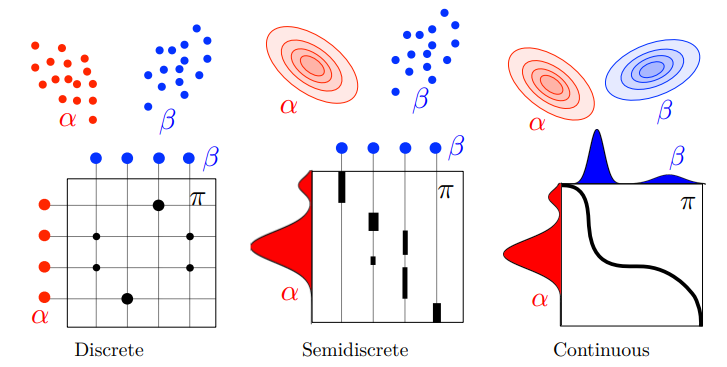
\includegraphics[width=0.6\textwidth]{png/3TypesOfOT.png}
            \vspace{-.7em}
            \caption{Three main scenarios for Kantorovich OT}
        \end{minipage}
        \begin{minipage}[t]{0.38\linewidth}
            \vspace{0pt}
            \centering
            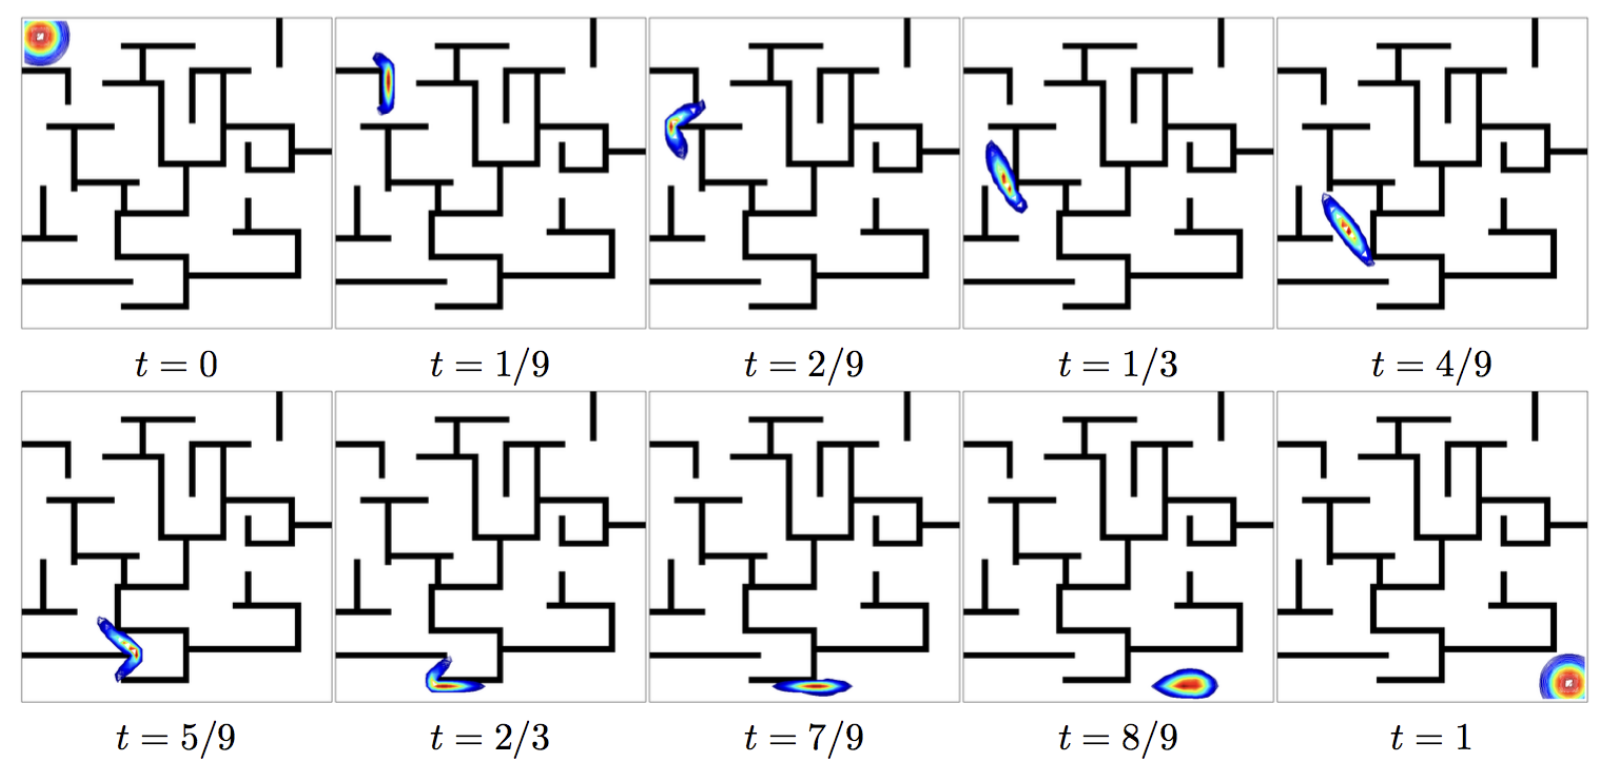
\includegraphics[width=0.98\textwidth]{png/maze.png}
            \caption{Solving maze with OT}
            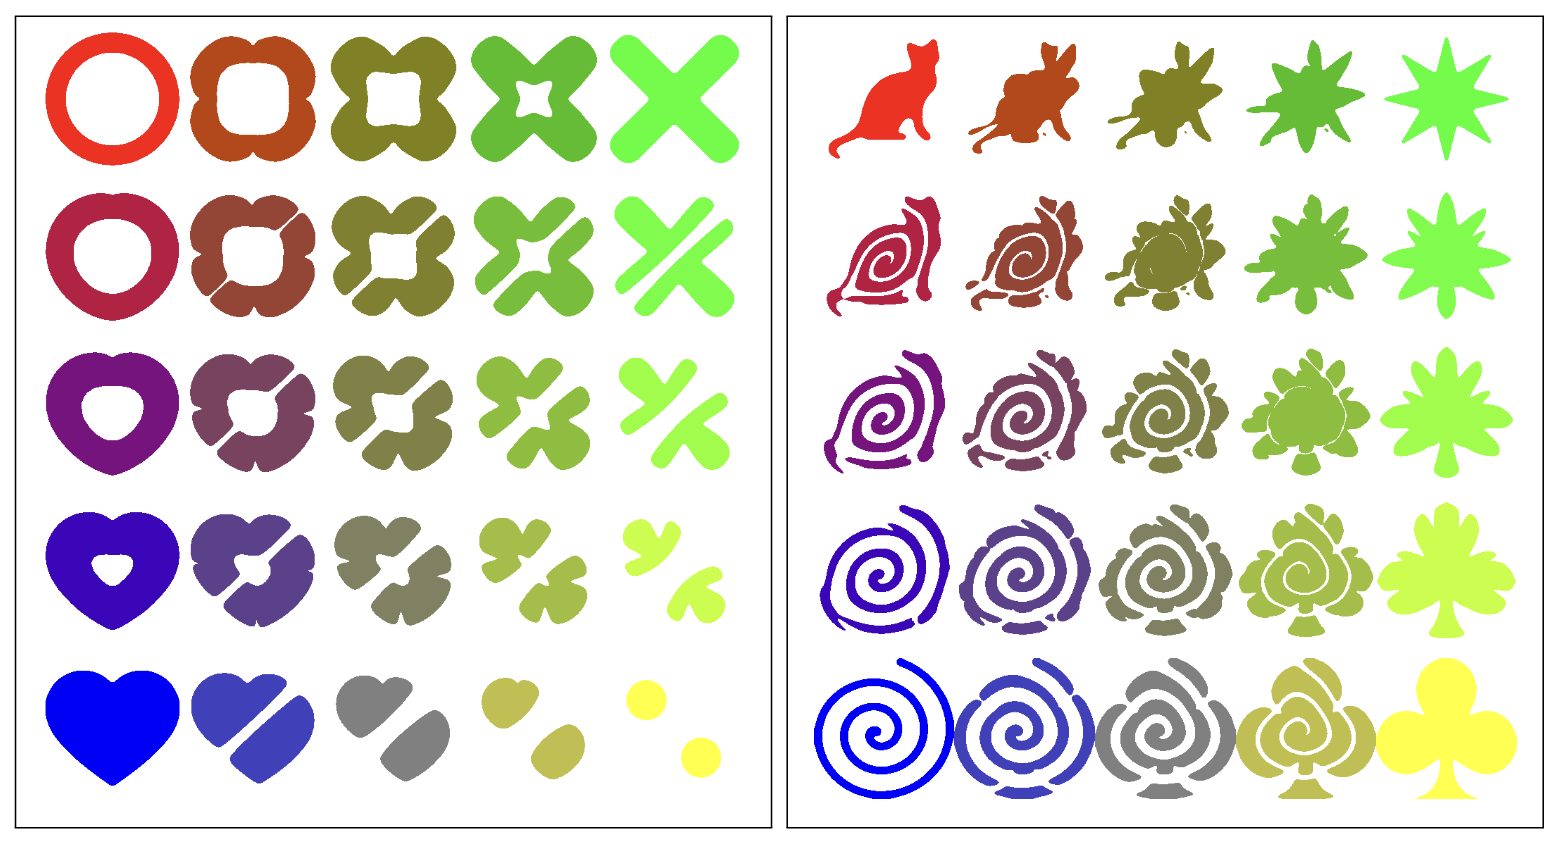
\includegraphics[width=0.98\textwidth]{png/2DShapeInterpolation.png}
            \caption{2D shape interpolation with OT}
            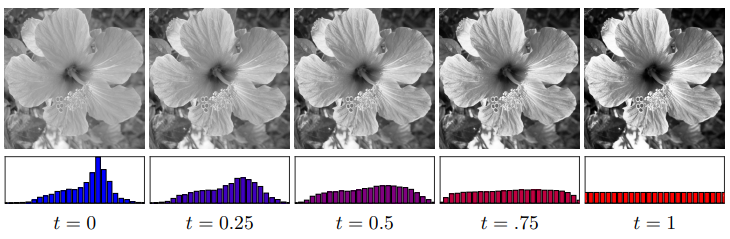
\includegraphics[width=0.98\textwidth]{png/HistogramEqualization.png}
            \caption{Histogram equalization with OT}
        \end{minipage}
    \end{figure}
\end{frame}

\begin{frame}
    \begin{center}
        {\Huge\calligra Thank You}
    \end{center}
\end{frame}

\end{document}